% Chapter 1

\chapter{Adiabatic quantum computing} % Main chapter title

\label{Chapter1} % For referencing the chapter elsewhere, use \ref{Chapter1} 
In the present chapter we discuss one of the paradigm of quantum computation known as \textit{adiabatic quantum computing} (AQC) which is hold by the adiabatic approximation that we discuss in further sections. The goal of the chapter is to show in detail the basis theory of the technique we use to solve TEP problems. Despite the chapter shows in detail each step of the theory it is not required for the reader to get a deeper understanding of it. To understand this dissertation is enough with the rough idea.
\section{Adiabatic approximation}
We start with the state $\ket{\psi(t)}$ of an $n$-qubit system whose Hamiltonian's $\mathcal{H}(t)$ spectrum is discrete and non-degenerate. The evolution of our state is given by the Schrödinger equation, see \ref{AppendixA},
\begin{equation}
    i\hbar \ket{\dot{\psi}(t)} = \mathcal{H}(t) \ket{\psi(t)}
\end{equation}
The time-independent solution for the Schrödinger equation for a discrete non-degenerate Hamiltonian is
\begin{equation}
    \mathcal{H}\ket{n(t)} = E_{n}(t)\ket{n(t)}
\end{equation}
where $\ket{n(t)}$ are the instantaneous eigenstates of the Hamiltonian and $E_{n}(t)$ are the eigenenergies labelled with the sub-indices $n$.\footnote{We can label the eigenenergies with a sub-index because the Hamiltonian is discrete and non-degenerate. If the Hamiltonian is just discrete we need an extra index to take into account the degeneration of each state, $E_{n}^{n_{i}}(t)$.}\\
We can re-write the Hamiltonian in diagonal form using the change-of-basis matrix $U(t)$,
\begin{equation}
    \mathcal{H}_{d}(t) = U^{-1}(t)\mathcal{H}(t)U(t) = \begin{bmatrix}
           \lambda_{0} & 0 & \hdots & 0 \\
           0 &  \ddots & & \vdots \\
           \vdots &   & \ddots & 0 \\
           0 & \hdots & 0 & \lambda_{2^{n-1}}
         \end{bmatrix}
\end{equation}
We also define $\ket{\psi_{d}(t)} = U^{-1}(t)\ket{\psi(t)}$ as the state we get after applying the inverse transformation $U^{-1}(t)$ to the initial state $\ket{\psi(t)}$.\\
Using the identity $\mathbb{I} = U(t)U^{-1}(t)$ in the equations and multiplying both sides by $U^{-1}(t)$ yields to
\begin{equation}
     i\hbar U^{-1}(t) \frac{\partial \left(U(t)U^{-1}(t)\ket{\psi(t)}\right)}{\partial t} = U^{-1}(t)\mathcal{H}(t) \left(U(t)U^{-1}(t)\right)\ket{\psi(t)}
\end{equation}
Manipulating terms
\begin{equation}
     i\hbar U^{-1}(t) \frac{\partial U(t)}{\partial t}\ket{\psi_{d}(t)} + i\hbar  \frac{\partial \ket{\psi_{d}(t)}}{\partial t}= \mathcal{H}_{d}(t)\ket{\psi_{d}(t)}
\end{equation}
%Rev
If we assume $\mathcal{H}(t)$ varies "slowly" -- in further sections we discuss what slowly means in detail -- then, it is reasonable that its change of basis $U(t)$ varies slowly too, $\dot{U}(t) \simeq 0$, which implies
\begin{equation}
    i\hbar  \frac{\partial \ket{\psi_{d}(t)}}{\partial t} \simeq \mathcal{H}_{d}(t)\ket{\psi_{d}(t)}
\end{equation}
The evolution of a state $\ket{\psi_{d}(t)}$ is lead by a diagonal Hamiltonian $\mathcal{H}_{d}$ so we have a set of non-coupled differential equations for each amplitude component of the state $\ket{\psi_{d}(t)}$. Furthermore, if the state of the system $\ket{\psi_{d}(t)}$ is an eigenstate of the Hamiltonian $\ket{n(t)}$, then, the evolution of our system is proportional to the eigensate $\ket{n(t)}$ so the evolution is lead inside the eigenspace of $\ket{n(t)}$ for a discrete non-degenerate Hamiltonian.
\begin{figure}[h]
    \centering
    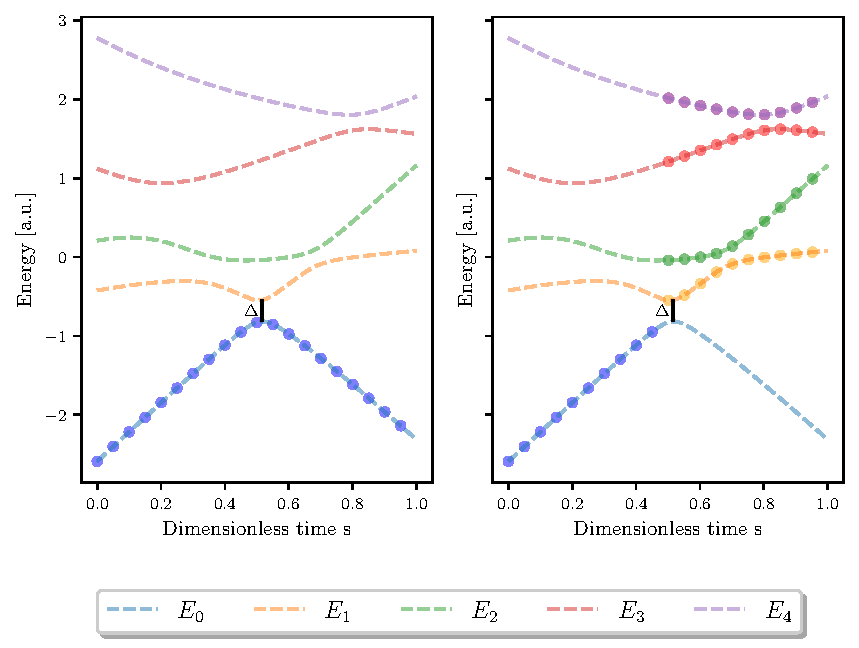
\includegraphics[width=\textwidth]{Figures/Eigenenergies.pdf}
    \caption{\textbf{INSERT CAPTION}}
    \label{fig:Eigenenergies}
\end{figure}
%%%%%%%%%%%%%%%%%%%%%%%%%%%%%%%%%%%%%%%%%%%%%%%%%%%%%%%%%%%%%%%%%%%%%%%%%%%%%%%%%%%%%%%%%%%%%%%%%%%%%%%%%%
%     1.2 ADIABATIC THEOREM
%%%%%%%%%%%%%%%%%%%%%%%%%%%%%%%%%%%%%%%%%%%%%%%%%%%%%%%%%%%%%%%%%%%%%%%%%%%%%%%%%%%%%%%%%%%%%%%%%%%%%%%%%%
\subsection{Adiabatic theorem}
Quoting Sarandy and Lidar,
\begin{displayquote}
\textit{The theorem posits, roughly, that if a state is an instantaneous eigenstate of a sufficiently slowly varying Hamiltonian at one time, then it will remain an eigenstate at later times, while its eigenenergy evolves continuosly.}
\end{displayquote}
We start by writing down the Schrödinger equation
\begin{equation}
    i\hbar \frac{\partial \ket{\psi(t)}}{\partial t} = \mathcal{H}(t)\ket{\psi(t)}
\end{equation}
Assuming the spectrum of $\mathcal{H}(t)$ is discrete and non-degenerate
\begin{equation}
\label{eq:Hamiltonian}
    \mathcal{H}(t) \ket{n(t)} = E_{n}(t)\ket{n(t)}
\end{equation}
Then, the eigenstates of the Hamiltonian -- which is an Hermitian operator -- form an orthonormal basis, so we can expand a given state in that basis
We can expand $\ket{\psi(t)}$ in term of the eigenvectors $\ket{n(t)}$
\begin{equation}
\label{eq: EigenvectorExpansion}
    \ket{\psi(t)} = \sum_{n}c_{n}(t)e^{i\theta_{n}(t)} \ket{n(t)}
\end{equation}
where
\begin{equation}
    \theta_{n}(t) = -\frac{1}{\hbar}\int_{0}^{t}E_{n}(t^{\prime})dt^{\prime}
\end{equation}
Substituting \ref{eq: EigenvectorExpansion} into the Schrödinger equation yields to
\begin{equation}
    \sum_{n}\left[\dot{c}_{n}(t)\ket{n(t)} + c_{n}(t)\ket{\dot{n}(t)}\right]e^{i\theta_{n}(t)} = 0
\end{equation}
Multiplying by $\bra{m(t)}$,
\begin{equation}
\label{eq:Coefficients}
    \dot{c}_{m}(t) = - \sum_{n}c_{n}\braket{m(t)|\dot{n}(t)}e^{i\left(\theta_{n}(t) - \theta_{m}(t)\right)}
\end{equation}
We can define $g_{nm}(t)\equiv E_{n}(t) - E_{m}(t)$ as the energy difference as function of time $t$ between the states $\ket{m(t)}$ and $\ket{n(t)}$.\\
We need to re-write $\braket{m(t)|\dot{n}(t)}$ in terms of the Hamiltonian's derivative. By deriving \ref{eq:Hamiltonian},
\begin{equation}
    \frac{\partial \mathcal{H}(t)}{\partial t}\ket{n(t)} + \mathcal{H}(t)\frac{\partial \ket{n(t)}}{\partial t} = \frac{\partial E_{n}(t)}{\partial t} \ket{n(t)} + E_{n}(t)\frac{\partial \ket{n(t)}}{\partial t} 
\end{equation}
Multiplying the last expression by $\bra{m(t)}$ 
\begin{equation}
    \braket{m(t)|\frac{\partial\mathcal{H}(t)}{\partial t}\ket{n(t)}} + E_{m}(t)\braket{m(t)|\dot{n}(t)} = E_{n}(t)\braket{m(t)|\dot{n}(t)}
\end{equation}
Finally,
\begin{equation}
    \braket{m(t)|\dot{n}(t)} = \frac{1}{E_{n}(t)-E_{m}(t)}\braket{m(t)|\frac{\partial \mathcal{H}(t)}{\partial t}n(t)}
\end{equation}
Substituting into \ref{eq:Coefficients},
\begin{equation}
\label{eq:GeneralCoefficientsNoadiabaticApprox}
    \dot{c}_{m}(t) = -c_{m}(t) \braket{m(t)|\dot{m}(t)} - \sum_{n\neq m} c_{n}\frac{\braket{m|\dot{\mathcal{H}}|n(t)}}{g_{nm}(t)}e^{i\left(\theta_{n}(t) - \theta_{m}(t)\right)}
\end{equation}
Adiabatic evolution is ensured if the coefficients $c_{n}(t)$ evolve independently from each other, i.e., if their dynamical equations do not couple. Mathematically,
\begin{equation}
    \max_{0 \leq \tau \leq T} \abs{\frac{\braket{m(t)|\dot{\mathcal{H}}(t)|\ket{n(t)}}}{g_{nm}(t)}{g_{nm}(t)}} \ll \min_{0\leq t \leq T} \abs{g_{nm}(t)}
\end{equation}
where $T$ is the total evolution time.\\ 
Under the adiabatic approximation the equation \ref{eq:GeneralCoefficientsNoadiabaticApprox} turns into
\begin{equation}
    \dot{c}_{m}(t) = -c_{m}(t)\braket{m(t)|\dot{m}(t)}
\end{equation}
The solution of the last equation is
\begin{equation}
    c_{m}(t) = c_{m}(0)e^{i\gamma_{m}(t)}
\end{equation}
where
\begin{equation}
    \gamma_{m}(t) = i\int_{0}^{t}\braket{m(t^{\prime}|\dot{m}(t^{\prime})}dt^{\prime} \quad \gamma_{m}\in \mathbb{R}
\end{equation}
%----------------------------------------------------------------------------------------

\section{Quantum annealing}

